
% ----------------------------------------------------------
% Introdução (exemplo de capítulo sem numeração, mas presente no Sumário)
% ----------------------------------------------------------

\chapter{Especificações para a proposta}

Os assuntos abordados nesta sessão procuram apresentar especificações sobre a proposta inicial do projeto, descrevendo os meios e resultados obtidos para a identidade visual, viabilidade e funcionalidades iniciais.

\section{Design da marca}

Cogitando a missão do projeto, surgiu a ideia de dar o nome \gls{ifriends} para o sistema, cuja origem é a junção de duas palavras: IF e \textsl{friends}. Isto devido a elas retratarem bem o âmbito que será atingido, já que tais palavras em conjunto transmitem o significado de ``amigos do \acs{ifsp}'', nome ideal para um projeto que visa tornar a interação dos alunos mais favorável.

A próxima etapa do desenvolvimento inicial da marca foi a elaboração de uma logo, assim como a definição das cores iniciais do sistema. A logo foi desenvolvida por meio do \gls{canva}, pois a plataforma se encontrava nos intermédios necessários para a elaboração da mesma. 

\begin{figure}[htb]
\centering
\caption{Logo do projeto}

\includegraphics[width=0.5\textwidth]{anexos/logo.png}
\fonte{Os autores.}
\end{figure}
\FloatBarrier

Já a seleção das cores iniciais do sistema traçou um caminho através de um estudo a respeito da psicologia das cores, visto que a equipe se preocupou em passar uma boa experiência até mesmo no quesito visual. Dessa forma, se definiu o azul e suas variações como a cor principal do sistema, já que segundo \citeonline{Tornos2021Sep}, os tons de azul se associam a princípios como: proteção, tranquilidade, fidelidade, compromisso, verdade, estabilidade, criatividade, entre outros. Vale ressaltar que o sistema ainda contará com outras cores, como roxo e algumas de suas variações, cores de sistema: variações de verde e vermelho, e cores neutras: variações de preto, cinza e branco.

Ainda, outro ponto considerado na criação da proposta foi a experiência do usuário final, pois mostrado assim como na \autoref{pesquisa}, a equipe se preocupou em estudar e conhecer melhor as dores deles. Visto que, segundo \citeonline{BibEntry2020Aug}, para tornar essa experiência agradável o sistema deve recorrer aos requisitos do modelo de colmeia desenvolvido por Peter Morville, sendo eles: útil, utilizável, desejável, acessível, confiável, localizável e valioso.

\begin{figure}[htb]
\centering
\caption{Modelo Colmeia}
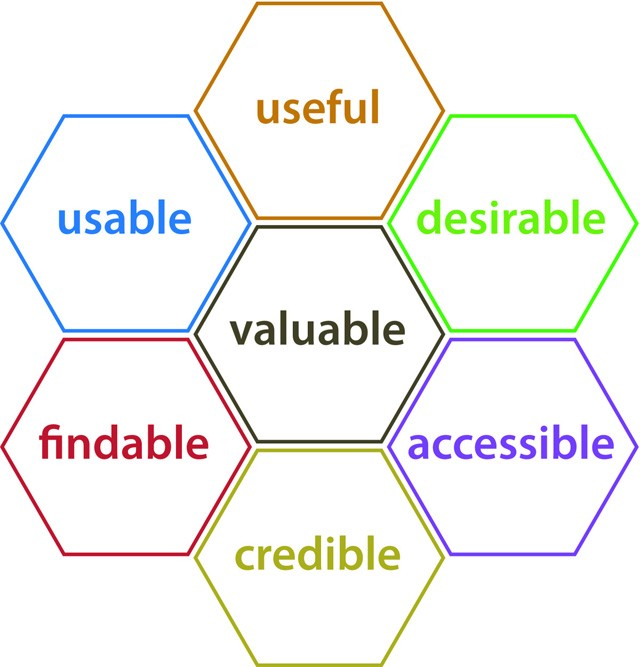
\includegraphics[width=0.4\textwidth]{anexos/modelo_colmeia.jpg}
\fonte{liferay.com}
\end{figure}
\FloatBarrier

%%%%%%%%%%%%%%%%%%%%%%%%%%%%%%%%%%%%%%%%%%%%%%%%%%%%%%%%%%

\section{Pesquisa de viabilidade} \label{pesquisa}
Foi realizada pela equipe uma pesquisa de viabilidade da aplicação, visando verificar se o público-alvo realmente estava sendo atingido, ou seja, se os alunos da instituição possuem interesse na aplicação e pretendem utilizar a mesma como ferramenta cotidiana para auxilia-los durante os estudos.

Para isto, houve a elaboração de um formulário por meio da ferramenta \gls{googleforms}, onde solicitamos que os alunos da instituição respondessem, com sinceridade, dez questões (\autoref{questões}) sobre a proposta. Sua divulgação ocorreu por meio do aplicativo de conversas \gls{WhatsApp}, onde os integrantes da equipe ficaram responsáveis por enviar o endereço de compartilhamento do formulário nos grupos de alunos conhecidos na instituição.

A realização desta pesquisa é de grande importância para a equipe avaliar a proposta que está sendo apresentada e para analisar sua viabilidade por meio dos resultados.
%%%%%%%%%%%%%%%%%%%%%%%%
\subsection{Resultados}

A partir deste formulário, foram recebidas quarenta e cinco respostas acumuladas dentro de um período de cinco dias, e ao final, foi possível constatar as seguintes características na maioria das respostas:

Algumas características do maior grupo que responderam ao questionário são: 

\begin{itemize}
    \item 86,7\% dos estudantes são do ensino médio integrado ao técnico;
    \item 66,7\% dos que sentiram dificuldade ao ingressar no \acs{ifsp}, compartilhou em forma de resposta curta suas experiências (como, adaptação com as atividades, dificuldades em matérias específicas, falta de transparência nas informações institucionais);
    \item 60\% nunca frequentaram ou vão raramente às monitorias;
    \item 85,5\% usariam o sistema e acreditam que o mesmo o ajudaria academicamente;
\end{itemize}

Com base nesses resultados, a equipe entende que a proposta cumpre seu objetivo de atingir os alunos do \acs{ifsp} com o desenvolvimento de uma comunidade de apoio aos assuntos enfrentados durante sua formação. Para pesquisas futuras, foi percebido, com base nas respostas, que uma melhoria na descrição das funcionalidades ajudaria o público-alvo a compreender melhor o objetivo da aplicação. Portanto, é possível validar, futuramente, dores dos usuários com pesquisas de usabilidade após melhores detalhamentos sobre o escopo do sistema.
%%%%%%%%%%%%%%%%%%%%%%%%%%%%%%%%%%%%%%%%%%%%%%%%%%%%%%
\section{Funcionalidades iniciais}

Através da pesquisa de viabilidade e das discussões feitas anteriormente pela equipe, foram elencadas algumas funcionalidades que poderão compor o escopo inicial do projeto, conforme apresentadas nessa sessão. 

\begin{itemize}
\item \textbf{Perguntar e responder questões}: Possibilitar que os usuários respondam e façam perguntas no fórum;

\item \textbf{Gamificação para ganho de reputação a cada reposta dada}: Possibilidade de votar positivamente nas respostas e de ganhar emblemas conforme o aumento da sua reputação;

\item \textbf{Trazer as perguntas mais relevantes na página inicial}: Exibir na página inicial para o usuário, as perguntas mais relevantes sobre temas específicos, tal relevância será considerada por meio da interação recebida. 

\item \textbf{Dividir as perguntas por categorias}: Serão predefinidas de antemão todas as possíveis categorias que podem chegar a ser necessárias na elaboração das perguntas, e caso chegue a faltar alguma, o usuário poderá fazer o uso da categoria ``outros'' que também estará disponível para suprir tal inconveniente. 

\item \textbf{Recorrer a \textit{tags}}: Para auxiliar as categorias, o usuário também poderá recorrer ao uso de \textit{tags}, as \textit{tags} seriam especificações a mais a respeito daquela categoria. Dessa forma, caso o usuário opte pela categoria ``Matemática'', dentro de suas \textit{tags} ele poderá definir, por exemplo, a matéria referente como ``Porcentagem''.

\item \textbf{Divulgação de monitorias no perfil do usuário}: O usuário terá uma seção no seu perfil para mostrar seus eventos de monitorias de determinados assuntos.

\end{itemize}


%%%%%%%%%%%%%%%%%%%%%%%%%%%%%%%%%%%%%%%%%%%%%%%%%%%%%%%%%%%%%%
